\chapter{Architecture}
Comme expliqué dans les chapitres précédent, nous avons construit notre application web sous forme de deux micro services :
\begin{itemize}
    \item Le frontend en lien direct avec l'utilisateur, l'interface graphique
    \item Le backend qui est le serveur du frontend et le client pour la base de données et ExaBGP.
\end{itemize}

\section{Frontend}
Afin de permettre à l'utilisateur d'accéder facilement aux différentes fonctionnalités du backend, nous avons déployé un frontend basé sur un serveur Django.

On ne détaillera pas trop cette architecture car elle n'est pas très important par rapport au backend et que notre architecture est fortement restreinte par le framework qui impose son style.

Ce frontend, se concentre sur la récupération des données stockées en backend, leurs mises en formes ainsi que les traitements lié aux besoins fonctionnel.

Lorsque le frontend souhaite échanger avec le backend, il peut utiliser les méthodes HTML:
\begin{itemize}
    \item [\textbf{GET api/subnet/id}] : pour obtenir une route
    \item [\textbf{GET api/subnets}] : pour obtenir toutes les routes
    \item [\textbf{POST api/subnets}] : pour créer une route
    \item [\textbf{PUT api/subnet/id}] : pour mettre à jour une route
    \item [\textbf{PATCH api/subnet/id}] : pour mettre à jour le statu d'une route
    \item [\textbf{DELETE api/subnet/id}] : pour supprimer une route\newline
\end{itemize}

Pour rendre l'interface utilisateur la plus agréable à utiliser possible, nous avons utilisé un framework Bootstrap "AdminLTE".

Les différents templates sont donc une extension du template de base d'AdminLTE. Ce framework nous permet donc de gérer facilement la mise en forme du "header", "footer" et de la "navbar".

Pour le style de certains éléments, nous avons intégré du css.

L'architecture du frontend est centré sur le fichier \verb+view.py+ qui permet de faire fonctionner notre application:
\begin{itemize}
    \item redirection
    \item gestion du tri
    \item récupération des données
    \item vérification de l'authentification
    \item utilisation des données renvoyées par les templates
    \item gestion des erreurs liées au frontend \newline
\end{itemize}

Nos différentes urls sont regroupée dans le fichier \verb+urls.py+.

La sécurité est gérée par le package de base de Django.

Toute les requêtes que nous enverrons à l'api ont été regroupée dans le fichier \verb+request\_json.py+. Ce fichier se trouve dans le dossier lié à notre application.

\section{Backend}

Cette fois-ci détailler l'architecture n'est pas trivial. C'est pourquoi, nous pouvons vous montrer le diagramme de classe du backend.

\begin{figure}[H]
    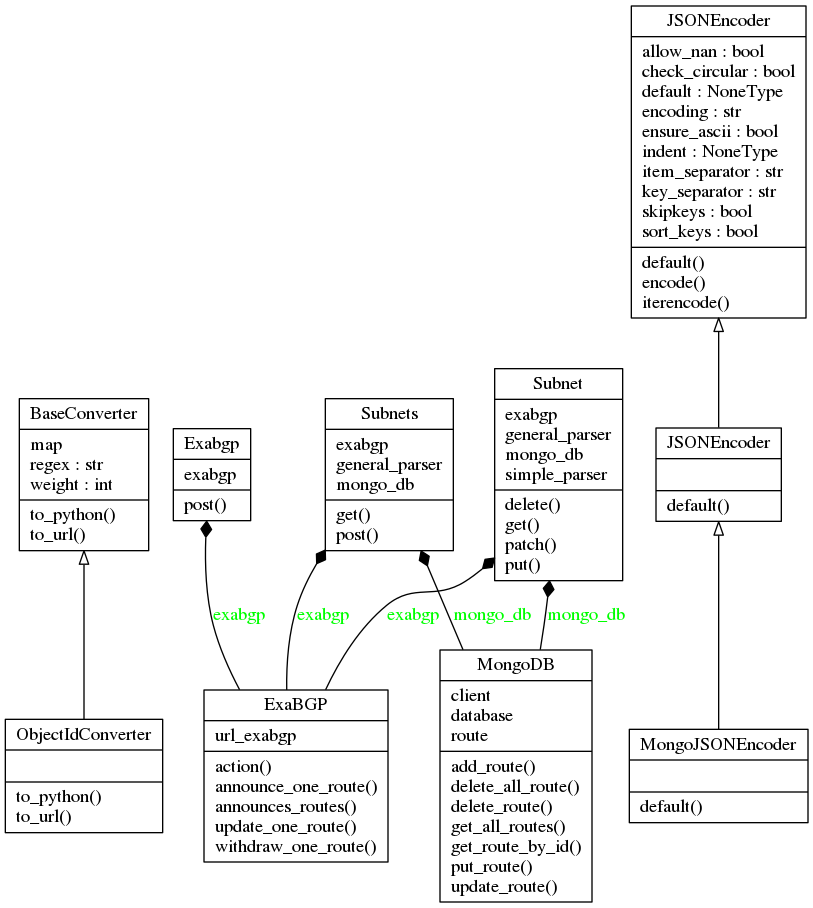
\includegraphics[width=\textwidth]{classes_backend.png}
    \caption{Diagramme de classe du backend}
    \label{fig:class_backend}
\end{figure}

Même si ce diagramme s'explique de lui-même, on va tout de même vous l'explique.

Il est constitué de différentes parties :
\begin{itemize}
    \item [\textbf{ExaBGP}] : le logiciel de gestion des routes
    \item [\textbf{MongoDB}] : sert de base de données
     \item [\textbf{API}] : permet de faire le lien entre les différents modules et le frontend
\end{itemize}

\subsection{ExaBGP}
Comme expliqué dans les \hyperref[sssec:exabgp]{besoins d'ExaBGP}, ce logiciel permet de gérer les routes d'un réseau régit par le protocole BGP.
L'API va donc par différentes méthodes interagir avec l'API de ExaBGP et permettre l'envoi et l'exécution de commande textuelles.

Cette ressource permet d'exécuter des commandes d'ExaBGP. Les commandes actuellement disponibles sur le frontend sont :
\begin{itemize}
    \item [\textbf{restart}] : relance ExaBGP,
    \item [\textbf{reload}] : recharge les configurations
    \item [\textbf{shutdown}] : ferme ExaBGP
    \item [\textbf{reset}] : vide la file d'attente des commandes non encore exécutées
    \item [\textbf{version}] : montre la version d'ExaBGP
\end{itemize}

\subsection{MongoDB}
Via Mlab, il sera utilisé pour gérer la base de données stockant les routes émises par l'API.
Quand une route est stockée un ID unique lui est attribuée. Cet ID permettra d'agir sur la route en question.

\subsection{API}
L'API possède 3 ressources :
\begin{itemize}
    \item \textbf{Subnets} : qui va traiter toutes les routes,
    \item \textbf{Subnet} : qui va traiter une seule route,
    \item \textbf{Exabgp} : utilisée pour envoyer des commandes à ExaBGP
\end{itemize}
\subsubsection{Subnets}
Cette ressource met à disposition les méthodes GET et POST pour le Frontend. En effet, celles-ci permettent respectivement d'afficher toutes les routes présentes dans la base de données et de créer une route au besoin de l'utilisateur. La route crée sera ajoutée à la base de donnée uniquement si la réponse d'ExaBGP est positive.
Si la réponse est négative, un message d'erreur est envoyé qui sera relayé par le Frontend pour en informer l'utilisateur.

\subsubsection{Subnet}
Cette ressource met à disposition les méthodes GET, PATCH, PUT et DELETE également pour le Frontend.

Grâce à un ID, préalablement récupéré, la méthode GET permet d'accéder aux informations concernant une route seulement.

Les méthodes PUT et PATCH permettent, quant à elles, de modifier une route déjà existante, toujours grâce à un ID.
PUT touchera à tous les champs de la route, alors que PATCH s'occupera simplement du champs "\textbf{is\_activated}", c'est-à-dire si la route est active ou non.

Pour faire la mise à jour de la route sur ExaBGP, elle sera préalablement supprimée et recréée avec les nouvelles modifications. Si échec, un message d'erreur est renvoyé.

La méthode DELETE permet la suppression de la route, qui est également envoyée à ExaBGP avec en retour un message d'erreur si échec.

\section{Diagramme de séquence}
\begin{figure}[H]
\caption{Diagramme séquentiel de l'ajout d'une route}
\fbox{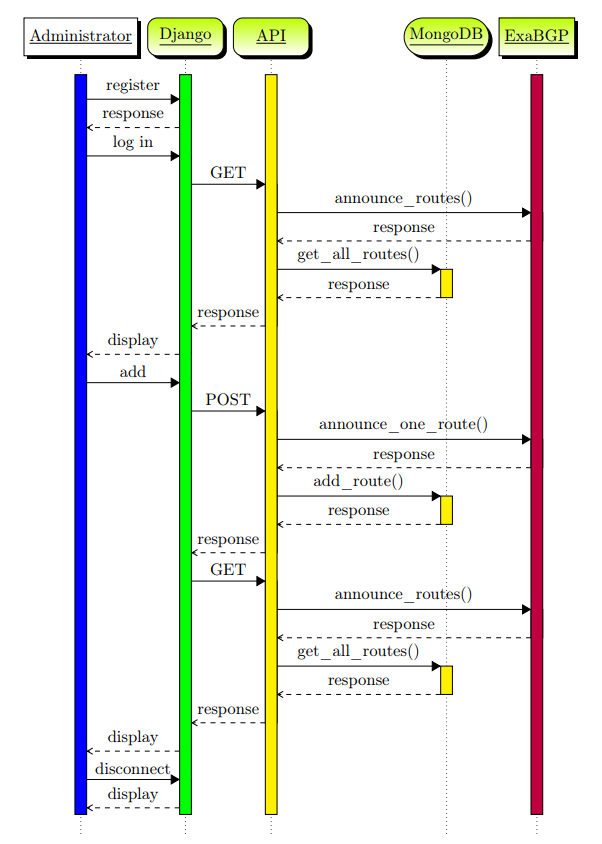
\includegraphics[width=\textwidth]{diagramme_seq.PNG}}
\label{fig:diagram_seq}
\end{figure}